\documentclass[tikz,border=10pt]{standalone}
\usepackage{mathpazo}
\usepackage{tikz}
\usetikzlibrary{shapes,arrows,positioning,calc,fit,backgrounds}

\begin{document}

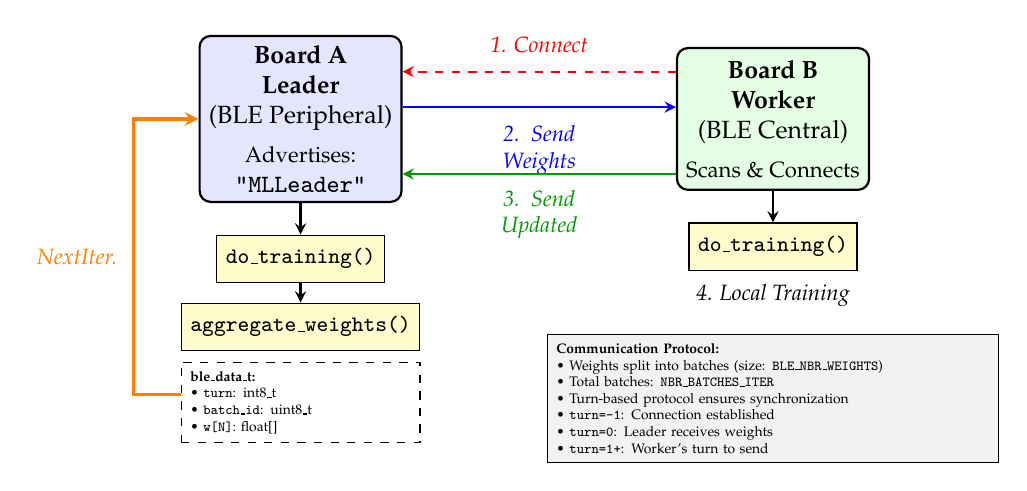
\begin{tikzpicture}[
    node distance=0.8cm,
    box/.style={rectangle, draw, thick, minimum width=2.2cm, minimum height=1.8cm, align=center, rounded corners, font=\small},
    leader/.style={box, fill=blue!10},
    worker/.style={box, fill=green!10},
    process/.style={rectangle, draw, fill=yellow!20, minimum width=1.8cm, minimum height=0.6cm, align=center, font=\footnotesize},
    arrow/.style={->, >=stealth, thick},
    dashedarrow/.style={->, >=stealth, thick, dashed},
    label/.style={font=\footnotesize\itshape}
]

% Board A (Leader)
\node[leader] (boardA) at (0,0) {
    \textbf{Board A}\\
    \textbf{Leader}\\
    (BLE Peripheral)\\[0.1cm]
    \footnotesize Advertises:\\
    \texttt{"MLLeader"}
};

% Board B (Worker)
\node[worker] (boardB) at (6,0) {
    \textbf{Board B}\\
    \textbf{Worker}\\
    (BLE Central)\\[0.1cm]
    \footnotesize Scans \& Connects
};

% Process boxes for Board A
\node[process, below=0.4cm of boardA] (trainA) {\texttt{do\_training()}};
\node[process, below=0.25cm of trainA] (aggA) {\texttt{aggregate\_weights()}};

% Process boxes for Board B
\node[process, below=0.4cm of boardB] (trainB) {\texttt{do\_training()}};

% Arrows showing communication flow
% Step 1: Initial connection (horizontal line at top, parallel to others)
\draw[dashedarrow, red] ($(boardB.west)+(0,0.6)$) -- node[above, label, yshift=3pt] {1. Connect} ($(boardA.east)+(0,0.6)$);

% Step 2: Send global weights (upper middle)
\draw[arrow, blue] ($(boardA.east)+(0,0.15)$) -- node[below, label, text width=1.8cm, align=center, yshift=-3pt] {2. Send\\Weights} ($(boardB.west)+(0,0.15)$);

% Step 3: Receive and train
\draw[arrow] (boardB) -- (trainB);
\node[label, below=0.05cm of trainB] {4. Local Training};

% Step 4: Send updated weights back (lower middle)
\draw[arrow, green!60!black] ($(boardB.west)+(0,-0.7)$) -- node[below, label, text width=1.8cm, align=center, yshift=-2pt] {3. Send\\Updated} ($(boardA.east)+(0,-0.7)$);

% Step 5: Aggregate
\draw[arrow] (boardA) -- (trainA);
\draw[arrow] (trainA) -- (aggA);

% Iteration loop indicator (points to left center of Board A)
\draw[arrow, thick, orange, line width=1.2pt] 
  ($(aggA.south west)+(0.2,-0.15)$) 
  -- ++(0,-0.4) 
  -- ++(-0.8,0) 
  |- (boardA.west) 
  node[pos=0.25, left, label, xshift=-2pt] {Next\\Iter.};

% Weight data structure annotation
\node[draw, dashed, fill=white, text width=2.8cm, align=left, font=\tiny, below=1cm of trainA] (data) {
    \textbf{ble\_data\_t:}\\
    • \texttt{turn}: int8\_t\\
    • \texttt{batch\_id}: uint8\_t\\
    • \texttt{w[N]}: float[]
};

% Legend box (bottom right, below Board B training box)
\node[draw, fill=gray!10, text width=5.5cm, align=left, font=\tiny, below=0.8cm of trainB.south] (legend) {
    \textbf{Communication Protocol:}\\
    • Weights split into batches (size: \texttt{BLE\_NBR\_WEIGHTS})\\
    • Total batches: \texttt{NBR\_BATCHES\_ITER}\\
    • Turn-based protocol ensures synchronization\\
    • \texttt{turn=-1}: Connection established\\
    • \texttt{turn=0}: Leader receives weights\\
    • \texttt{turn=1+}: Worker's turn to send
};

\end{tikzpicture}

\end{document}